\section{Discussion}\label{sec:disc}

\begin{figure}
\centering
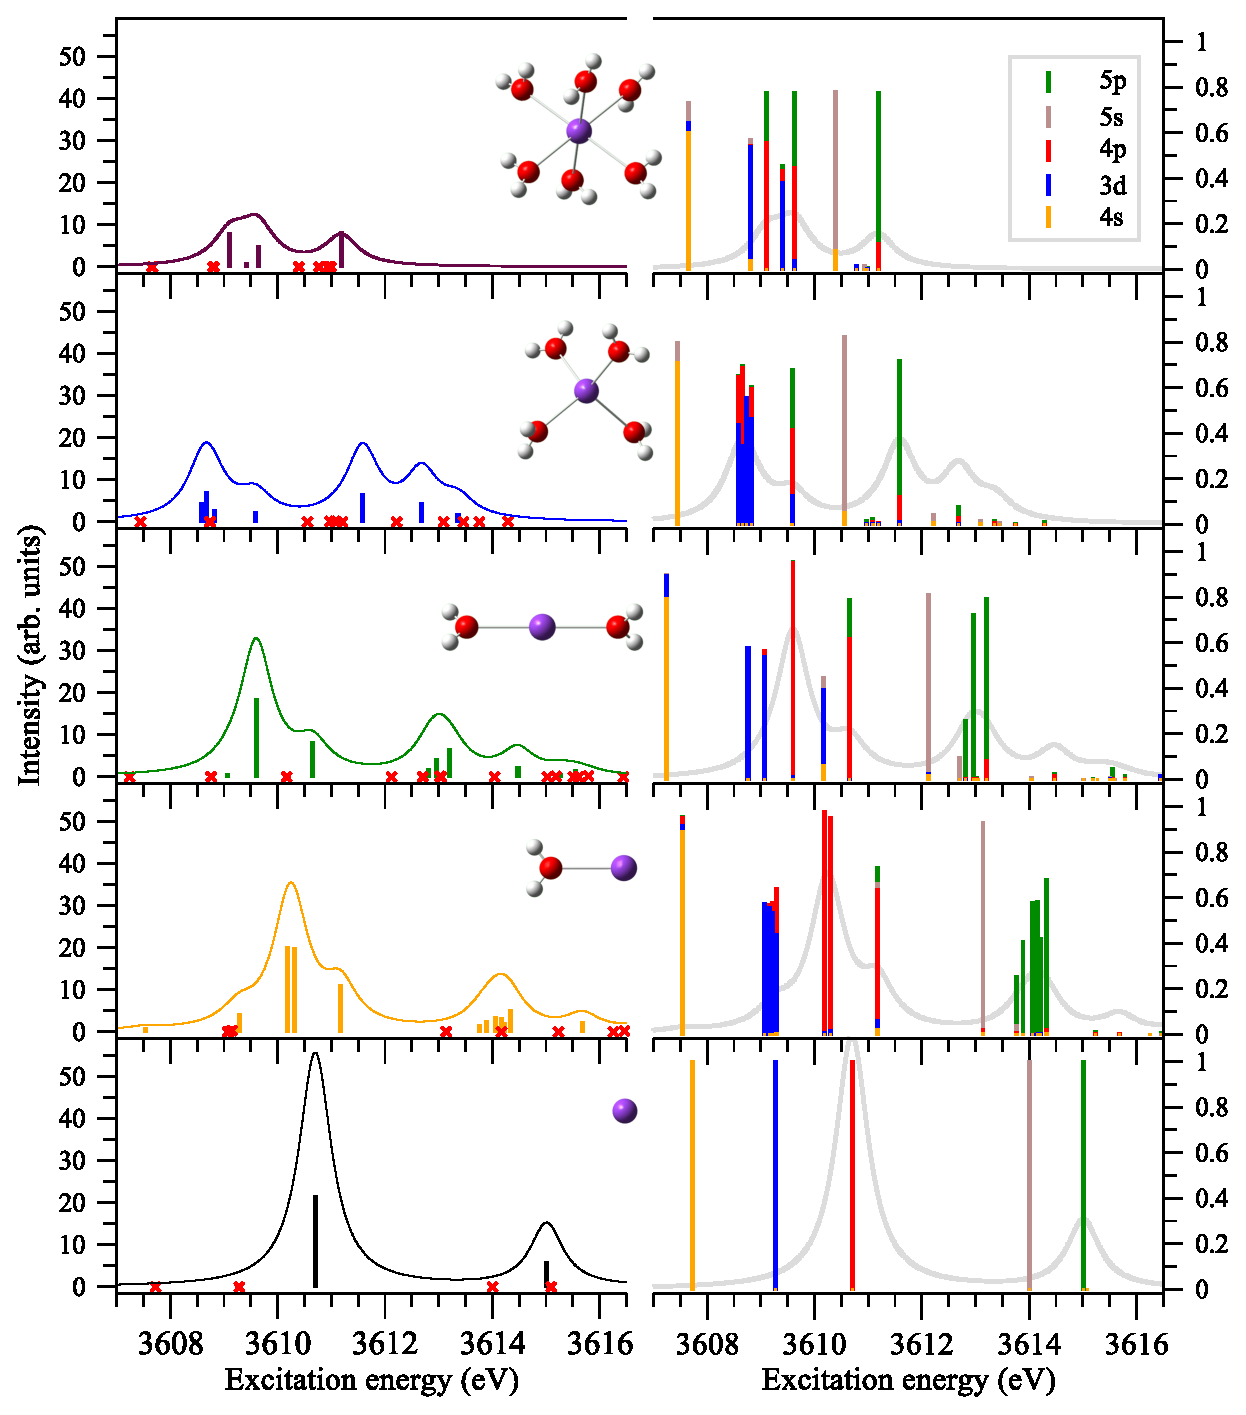
\includegraphics[scale=0.6]{figures/fg1_kh2on_xas_overlaps.eps}
\caption{Left panel: XAS spectra of the lowest core-to-valence and core-to-Rydberg transitions in the bare K$^{+}$ ion, and the microsolvated clusters K$^{+}$(H$_2$O)$_m$, $m = 1, 2, 4, 6$, computed at the CVS-ADC(2)x level of theory. The theoretical stick spectra were convolved with a Lorentzian profile of FWHM 0.74 eV in order to account for the lifetime broadening. Right panel: Projections $|a_{nl}^{i}|^2$ of the SONOs corresponding to the core excited states of the K$^{+}$(H$_2$O)$_m$ clusters with $m = 1, 2, 4, 6$ on the basis of SONOs corresponding to the 1s$\,\rightarrow\,$4s, 1s$\,\rightarrow\,$3d, 1s$\,\rightarrow\,$4p, 1s$\,\rightarrow\,$5s and 1s$\,\rightarrow\,$5p states in K$^+$ (see Eq.\ \eqref{eq:sono_proj}).
The theoretical X-Ray absorption spectra were shifted to higher photon energies by 6.7\,eV, which corresponds to the difference between the computed and experimental core excitation energies of the 1s $\rightarrow$ 4p excitation in the bare ion taken from Ref.\ \citep{hertlein06:062715}.}
\label{fg:knw_xas}
\end{figure}


\begin{figure}
\centering
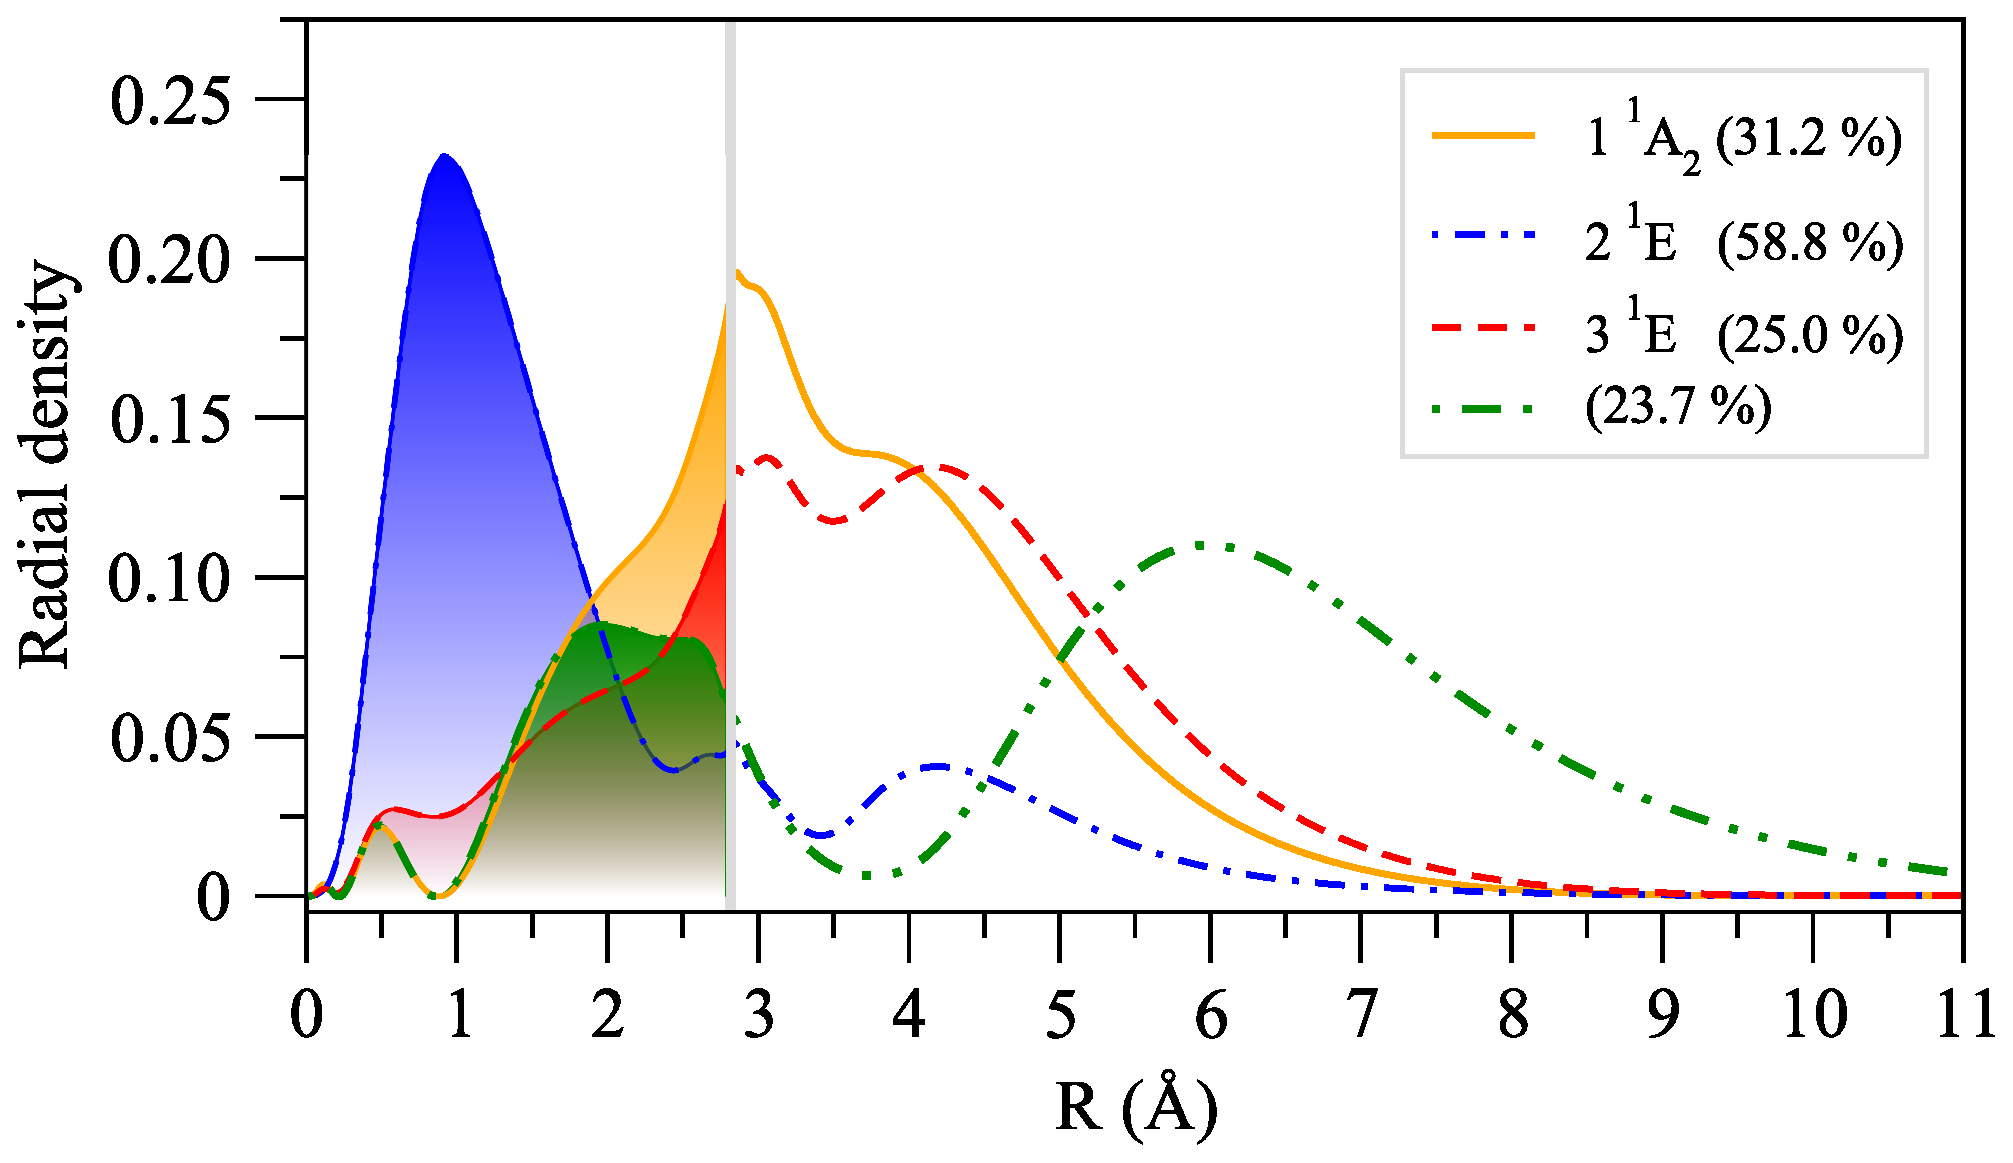
\includegraphics[scale=0.3]{figures/fg2_k_6w_okxx_55_rad_dens.eps}
\caption{Radial density distributions of the singly-occupied natural orbitals occupied by the excited electron in the core excited states 3609.11\,eV (1\,$^{1}$A$_{2}$), 3609.41\,eV (2\,$^{1}$E) and 3609.64\,eV (3\,$^{1}$E) of K$^{+}$(H$_2$O)$_6$. The grey line at 2.816\,\AA~represents the equilibrium K-O distance.}
\label{fg:rad_dens}
\end{figure}



\begin{figure}
\centering
\includegraphics[scale=0.6]{figures/clnw_xas.eps}
\caption{Left panel: XAS spectra of the lowest core-to-valence and core-to-Rydberg transitions in the bare \cli~ion, and the microsolvated clusters \cli(H$_2$O)$_m$, $m = 1, 2, 4, 6$, computed at the CVS-ADC(2)x level of theory. The theoretical stick spectra were convolved with a Lorentzian profile of FWHM 0.62 eV in order to account for the lifetime broadening (REF). Right panel: Projections $|a_{nl}^{i}|^2$ of the SONOs corresponding to the core excited states of the \cli(H$_2$O)$_m$ clusters with $m = 1, 2, 4, 6$ on the basis of SONOs corresponding to the 1s$\,\rightarrow\,$4s, 1s$\,\rightarrow\,$3d, 1s$\,\rightarrow\,$4p, 1s$\,\rightarrow\,$5s and 1s$\,\rightarrow\,$5p states in \cli~(see Eq.\ \eqref{eq:sono_proj}).}
\label{fg:clnw_xas}
\end{figure}


In order to understand the resonant Auger features in the experimental XAS/AES spectra we computed the X-ray absorption spectra of both \cli and \ki~and their microsolvated clusters with 1, 2, 4 and 6 water molecules, as well as the final Auger states for the bare ions.


%\begin{enumerate}
%\item XAS spectra of Cl$^{-}$ and K$^{+}$

%1.1 Bare ions: which states are dipole allowed in the bare ions? -- 1s$\,\rightarrow np$ excitations

Since we consider K-shell excitations, the optically allowed transitions in an isolated ion are to $p$-type virtual states. Thus, the states which will be observed upon photoexcitation will be 1s$\,\rightarrow np$ states \citep{hertlein06:062715} (ADD MORE REFS). Consequently, as can be seen from the XAS spectra of the bare ions on Figs.\ \ref{fg:knw_xas} and \ref{fg:clnw_xas}, the first observed peak corresponds to the 1s$\,\rightarrow\,$4p states. It is noteworthy that the positions of the 1s$\,\rightarrow\,$4p and 1s$\,\rightarrow\,$3d states are inverted in \cli and \ki. In the case of Cl$^{-}$ the 1s$\,\rightarrow\,$4p excitation has lower energy and the 1s$\,\rightarrow\,$3d excitation is close to the 1s$\,\rightarrow\,$5p state. On the contrary, in K$^{+}$ the 1s$\,\rightarrow\,$3d excitation has lower energy and lies below the 1s$\,\rightarrow\,$4p state. As we will see later, this implies that in \ki the 1s$\,\rightarrow\,$3d and 1s$\,\rightarrow\,$4p excitations can mix due to symmetry breaking in the ligand field of the water molecules similarly to the case of Na$^{+}$ and Mg$^{2+}$ (SOME REFERENCE HERE?)\citep{miteva16:16671}.


Another important observation is that the intensity of the 1s$\,\rightarrow\,$4p state is lower than that of the 1s$\,\rightarrow\,$5p state in \cli, contrary to what one would expect for a Rydberg series \citep{hussain07:022710}(MORE REF?) and contrary to what is observed for \ki. This phenomenon can be understood by the more compact radial density distribution of the excited electron in the 1s$\,\rightarrow\,$5p state compared to that of the 1s$\,\rightarrow\,$4p state shown in Fig.\ \ref{fg:rdens_ions} in Supporting Information. As a result of this, the overlap between the core electron and the more compact 5p orbital becomes larger, and thus the oscillator strength of the transition.


%1.3 Bare ions: comparison with literature


In Ref.\ \citep{hertlein06:062715}, the XAS spectrum of K$^{+}$ is measured. The ionic core excited states close to threshold are the 1s$\,\rightarrow\,$4p and 1s$\,\rightarrow\,$5p excitations at energies 3610.7\,eV and 3615.0\,eV, respectively. The experimental ionization potential of the bare ion, 3619.4\,eV, as well as the positions of the K-shell core excitations were determined using the core-equivalent approximation by a comparison between the experimental XAS spectrum of \ki and the valence-excitations of Ca$^{+}$. In a solution, due to the charge-dipole interaction between the metal ion and water molecules, as well as XXX interaction, one can expect a shift of the energies of the core excited states and the ionization potential, but also splitting and mixing of the states of the bare ion. Since in the bare ion one observes excitations up to 1s$\,\rightarrow\,$5p, also in a solution one cannot expect to observe core excited states higher than the 1s$\,\rightarrow\,$5p excitation, because the ionic state will be more stabilized in a solution compared to the core-excited states, and thus the difference in IPs will be larger than the difference in excitation energies.


\begin{table}
\begin{tabular}{c c c c}
\hline\hline
& \multicolumn{2}{c}{K$^{+}$} & K$^{+}_{\texttt{aq}}$ \\
\hline
& Ref.\ \citep{hertlein06:062715} & this work & this work \\
1s$\,\rightarrow\,$4p & 3610.7 (-8.7)& 3604.0 (-8.25 edge) & 3610.5 (Denis?)\\
1s$\,\rightarrow\,$5p & 3615.0 (-4.4) & 3608.31 (-3.94 from edge) & \\
Edge & 3619.4 & 3612.25 ($\Delta$SCF) & 3612 \\
\hline
\end{tabular}
\caption{XXX}
\end{table}


%1.4 Solvated clusters:

%splitting of the peaks (200meV between 1s -> 4p excitations in K+), and mixing of the core-excited states in the crystal field created by the solvent; intensity drops compared to the bare ions; dipole forbidden states such as 1s -> 3d core excitations mix with the dipole allowed 1s -> 4p states and acquire intensity

Upon the addition of water molecules, the core excited states in both \ki~and \cli~change. In particular, due to the ligand field of the water molecules, the degeneracy of the core excitations is lifted and they split into a number of states. Moreover, their intensity drops compared to the case of the bare ion. Additionally, the presence of the solvent molecules leads to mixing of the states of the bare ion. As a result, states which are dipole forbidden in the bare ion can acquire intensity in the microsolvated cluster.


Let us first consider the case of \ki~(see Fig.\ \ref{fg:knw_xas}). Upon the addition of a single water molecule, the 1s$\,\rightarrow\,$4p excitation splits into 2 lower lying states and a higher lying state separated by about 1\,eV. The same situation is observed in the doubly-coordinated cluster. In the 4-coordinated \ki~cluster, the first peak in the spectrum is produced by states which have a large contribution (0.5?) from the dark 1s$\,\rightarrow\,$3d states and a smaller contribution from the closely lying dipole allowed 1s$\,\rightarrow\,$4p core excitation. Finally, in the 6-coordinated cluster, which represents the complete first solvation shell around \ki, the first peak in the spectrum contains the 1s$\,\rightarrow\,$4p states split by approximately 0.5\,eV, and a state in between, which has predominantly 1s$\,\rightarrow\,$3d character.


The XAS spectra of the microsolvated clusters of \cli~are different due to the different electronic structure of the ion and the orientation of the surrounding solvent molecules. The water molecules tend to gather on one side of the \cli~ion and form H-bonds with it (REF). The resulting structures are of lower symmetry compared to the respective microsolvated clusters of \ki. Consequently, the higher lying core excited states completely lose their atomic character as can be seen from the right panel on Fig.\ \ref{fg:clnw_xas}. As one can see, only the lowest lying 1s$\,\rightarrow\,$4p excitation can still be distinguished in the microsolvated clusters. Unlike in the case of \ki, this state does not interact so strongly with the 1s$\,\rightarrow\,$3d state because they do not lie close in energy in the bare ion. The higher lying 1s$\,\rightarrow\,$5p states completely lose their atomic character, the second peak observed in the XAS spectrum of \cli~decreases in intensity and splits into multiple low-intensity peaks. In \cli~one cannot understand the splitting of the states as a simple electrostatic interaction between the ion and the ligands.

Since the calculation of the ionization threshold cannot be carried out at the same level of theory as the core excited states, one cannot determine which core excited states undergo resonant Auger decay. We can, however,  make an assumption by comparing the pre-edge structure in the experimental spectrum with the theoretical XAS spectrum. The pre-edge structure in the experimental XAS spectra shown on Figs.\ \ref{fg:2dmap_k} and \ref{fg:2dmap_cl} consists of a single peak and spreads within approximately 3\,eV below the ionization threshold. Upon observation of the theoretical XAS spectra one sees that this is approximately the width of the first peak in the 6-coordinated spectra of both \ki~and \cli. This peak is formed of states of predominantly 1s$\,\rightarrow\,$4p character in the case of \cli, and mixed 1s$\,\rightarrow\,$4p,3d,5p character in the case of \ki.


%{\color{red}The ionization potential in solution drops by XX\,eV, whereas the energy of the first core excited state only by YY\,eV, because the ionic state is more stabilized in a solution compared to the excited one.}

%On Fig.\ \ref{fg:rad_dens} we present the radial density distributions of the SONOs occupied by the excited electron in K$^{+}$(H$_2$O)$_6$. 

However, solely from the XAS spectra, one cannot extract information about the subsequent Auger process. As can be seen on the 2D maps of \ki~and \cli~and as discussed in the previous section, the resonant Auger process is the decay pathway of the lowest lying core excited states. In the case of 

The formation of such an island on the 2D map of \ki$_{\text{aq}}$ can result from several processes: shake-up resonant Auger decay, similar to the case of Ar \citep{ceolin15:022502}, spin-orbit splitting in the final states, or population of dipole forbidden states, which is a result of symmetry breaking in the presence of the solvent. 

\begin{enumerate}

\item[a)] Shake-up resonant Auger decay

A separate island at 2666\,eV kinetic energy and 3203.5\,eV photon energy is observed on the 2D map of Ar (see Fig.\ 2 in \citep{ceolin15:022502}. This island results from resonant Auger decay of the Ar 1s$\,\rightarrow\,$4p state to Ar$^{2+}$(2p$^{-2}$4p) states. The 1s$\,\rightarrow\,$4p state undergoes also shake-up resonant Auger decay, resulting in the population of Ar$^{2+}$(2p$^{-2}$5p) states which appear as a separate feature at the same photon energy, but at lower kinetic energies, 2662\,eV.


A similar shake-up decay can be expected for the 1s$\,\rightarrow\,$4p state of \ki. As a first step, we estimate the splitting between the 2p$^{-2}$4p and 2p$^{-2}$5p final states. Using the $(Z+2)$-approximation, the splitting between the 2p$^{-2}$4p and 2p$^{-2}$5p states of K$^{3+}$ is equal to the splitting between the 3p$^6$4p and 3p$^6$5p states of Sc$^{3+}$. From the NIST database \citep{NIST_ASD} for the bare ion we obtain $\sim$8.2\,eV, which agrees with the splitting between the island and the dispersive feature close to the $^1$D main line on the 2D map of \ki$_\text{aq}$ (Fig.\ \ref{fg:2dmap_k}). As a second step, we compare the intensity ratio between the two dispersive features in \ki$_{\text{aq}}$ with that in Ar. As can be seen from Fig.\ \ref{fg:intensity_ratio} the lower-lying peak, which is attributed to the K$^{3+}$(2p$^{-2}$5p) state has higher intensity compared to the higher-lying peak. The intensity of the two peaks in Ar is exactly the opposite implying a lower shake-up probability. Another counterargument against the shake-up origin of the island is that if one compares the maxima of the two dispersive features B and C, one sees that the feature B appears at lower photon energies than C. This is opposed to Ar, where the island originating from normal Auger decay appears at lower photon energies.

Another question is whether the 2p$^{-2}$5p states can be populated in a solution. To address this issue, on Fig.\ \ref{fg:k_2p4nl_raddens} we compare the radial density distributions of the natural orbitals occupied by the excited electron in the K$^{3+}$(2p$^{-2}$4p) and K$^{3+}$(2p$^{-2}$5p) states. The former distribution is quite compact, with 86\% of the electron density within the first solvation shell, whereas only about 20\% of the electron density in the  K$^{3+}$(2p$^{-2}$5p) state is within the first solvation shell.


Therefore, we conclude that the features B and C on the 2D map of \ki$_{\text{aq}}$ Fig.\ \ref{fg:2dmap_k} are not a result of a shake-up and normal Auger decay of the \ki(1s$\,\rightarrow\,$4p) state.


\item[b)] Spin-orbit splitting of the final states: it cannot give such a big difference (of 8\,eV)

{\color{red} Here I don't really know what to write}


\item[c)] Population of dipole forbidden states which results from symmetry breaking in the presence of the solvent


\begin{figure}[h!]
\centering
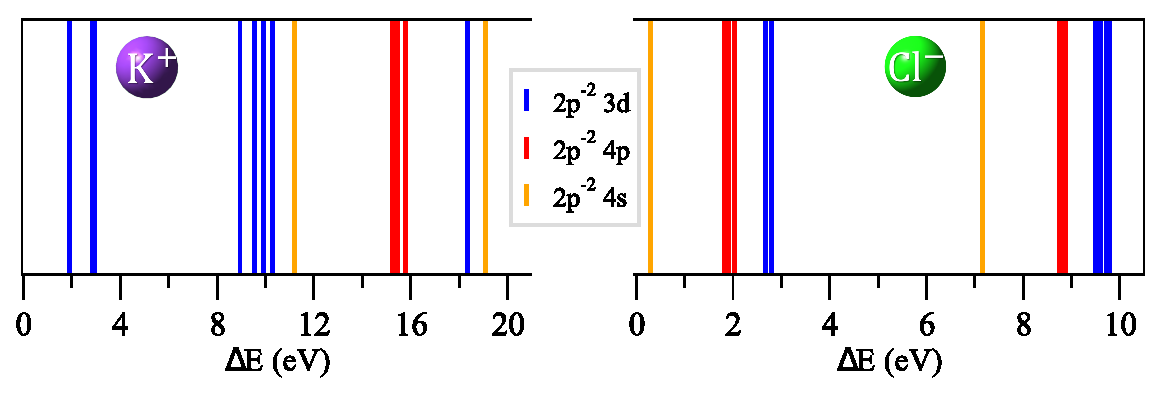
\includegraphics[scale=0.6]{figures/fg3_kcl_2p-2nl.eps}
\caption{Final 2p$^{-2}$($^3$P, $^1$D) 3d, 4s, 4p doublet Auger states of K$^{+}$ (left) and Cl$^{-}$ (right) computed at the CIS level (see Sec.\ \ref{sec:methods} for details). The states are shifted with respect to the lowest quartet state with electron configuration 2p$^{-2}$($^3$P) 4s.}
\label{fg:kcl_2p4nl}
\end{figure}


As discussed above, the addition of water molecules results in lifting of the degeneracy of the core-excited states and mixing. The latter results in the fact that dipole forbidden states such as the 1s$\,\rightarrow\,$3d excitation in \ki~acquire intensity in the XAS spectrum (Fig.\ \ref{fg:knw_xas}). The resonant Auger decay of these states can therefore result in the population of 2p$^{-2}$3d states. In what follows we analyze the final Auger states of \ki~and \cli. The final Auger states 2p$^{-2}$($^3$P, $^1$D)nl of \ki~and \cli~computed at the CIS level are presented on Fig.\ \ref{fg:kcl_2p4nl}. From all final states we plot only the doublets, because the quartet states are populated with very low probability (REFS). Already at the level of the bare ion one can see that the 2p$^{-2}$nl states of \ki~and \cli~are substantially different. First of all, the lowest doublet states of \ki, are of 2p$^{-2}$3d character, whereas the lowest states in the case of \cli~are 2p$^{-2}$4s followed by 2p$^{-2}$4p. Second, the 2p$^{-2}$nl states of \ki~appear in groups which are well separated from one another. The 2p$^{-2}$3d states are in 3 groups, located around 2, 10 and 18\,eV. The 2p$^{-2}$4p states, on their turn, appear around 15-16\,eV, and are well separated from the 2p$^{-2}$3d states by 5 and 12\,eV, respectively. Therefore, if the initial core-excited states are of mixed 1s$\,\rightarrow\,$3d and 1s$\,\rightarrow\,$4p character, in the Auger electron spectrum, one will observe an island corresponding to the 2p$^{-2}$3d states, separated from the main line, which will contain a dispersive feature formed as a result of the population of the 2p$^{-2}$4p states.


The situation in the case of \cli~is quite different. The 2p$^{-2}$3d and 4s states are not so well separated, but rather they form two groups of 2p$^{-2}$($^3$P)4p,3d and 2p$^{-2}$($^1$D)4p,3d states located around 2 and 9\,eV, respectively. Thus, even if the initial core-excited states are mixed 1s$\,\rightarrow\,$3d and 1s$\,\rightarrow\,$4p states of the bare ion, one will not observe separate dispersive features from the 2p$^{-2}$3d and 4p final states.

Another argument, supporting this hypothesis is that the intermediate state in the XAS spectrum of \ki(H$_2$O)$_6$ lies between the 1s$\,\rightarrow\,$4p excitations. Consequently, the dispersive feature in the Auger electron spectrum originating from its decay will appear at higher photon energies than the one originating from the decay of the 1s$\,\rightarrow\,$4p excitations, which is exactly the case of the island C and the feature B shown on Fig.\ \ref{fg:2dmap_k}. Moreover, the splitting between the maxima of B and C is of $\sim$400\,meV, which coincides with the splitting between the first 1s$\,\rightarrow\,$4p and the 1s$\,\rightarrow\,$3d excitations in the theoretical spectrum of the 6-coordinated cluster (Fig.\ \ref{fg:knw_xas}).

In the theoretical spectrum one can see that the intensity of the 1s$\,\rightarrow\,$3d state is much lower than that of the 1s$\,\rightarrow\,$4p states. Consequently, the fingerprint of this former state in the Auger electron spectrum will be of lower intensity compared to the latter one. This is in compliance with the experimental intensity of the island C which is lower than that of B (see Fig.\ \ref{fg:intensity_ratio}).

Consequently, we can conclude that the island C on the 2D map of \ki~Fig.\ \ref{fg:2dmap_k} is a result of the resonant Auger decay of a core excited state of the hydrated ion which has a dipole forbidden 1s$\,\rightarrow\,$3d character.


\end{enumerate}


{\color{blue}\bf Discuss the possibility for non-local Auger decay!}